% !TEX root = ./../main.tex
\chapter{Introduction to Molecular Dynamics}
For macroscopic bodies, the motion of a system in time and space is governed by the classical equations of motion, say the Newton’s law, while reducing time and space scales, quantum mechanics kicks in. Despite the latter statement, classical laws of motion have proved to be a good approximation also at the molecular level, as long as atoms are massive enough.

In order to predict the time evolution of a complete system, such as the biomolecular system we will treat in this thesis, Newton’s equations of motion need to be integrated numerically. The necessity of a numerical integration arises from the complexity of the interactions involved in realistic systems, often nonlinear functions of positions and momenta of the particles making up the system, which makes it impossible to obtain an analytical solution for the equations of motion.

In the first part of this Chapter the laws of classical and statistical mechanics will be briefly summarized. Then we introduce the computational \ac{MD} method and analyze the main aspect of this technique.

\section{Review of classical and statistical mechanics}
\subsection{Classical mechanics}
The classical behavior of a system of $N$ particles with mass $m_i$ and coordinates $\vec r_1,\cdots,\vec r_N$, is described by the Newton's second law. Each particle in the system will experience the total force $\vec F_i$ and the then the second law for particle $i$ yield
\begin{equation}
	m_i \ddot{\vec{r}}_i = \vec F_i(\vec r_1,\cdots,\vec r_N)
	\label{eq:newtonLaw}
\end{equation}

The total force is defined as
\begin{equation}
	\vec F_i(\vec r_1,\cdots,\vec r_N) = \vec{f}_i^{\ (e)}(\vec r_i) + \sum_{i\ne j}^N \vec{f}_{ij}^{\ (i)}(\vec r_i - \vec r_j )
\end{equation}
where $\vec{f}_i^{\ (e)}$ is the external force acting on particle $i$; while $\vec{f}_{ij}^{\ (i)}$ is the inter-particle force that $i$ exerts on $j$ and \textit{vice-versa}, in general it depends only on the distance between the particles. The equations~\eqref{eq:newtonLaw} is refereed to as \textit{the equations of motion} of the system; integrating them, with the sets of the \textit{initial conditions} at start time $t_0$: $\vec r_1(t_0),\cdots,\vec r_N(t_0)$ and $\dot{\vec{r}}_1(t_0),\cdots,\dot{\vec{r}}_N(t_0)$, the positions and the velocities of all the particles in the system at any time it is known.

An other way to write the equations of motion is to use the particles momenta $\vec p_i = m_i \dot{\vec{r}}_i$ and then the equations~\eqref{eq:newtonLaw} became
\begin{equation}
	\frac{d\vec p_i}{dt} = \vec F_i(\vec r_1,\cdots,\vec r_N)
	\label{eq:newtonLawMom}
\end{equation}
Obtain the full set of $6N$ functions $\{\vec r_1(t),\cdots,\vec r_N(t),\vec p_1(t),\cdots,\vec p_N\}$ give us a full description of the dynamics of the $N$--particle system. The set of functions above can be arranged in an ordered $6N$--dimension vector
\begin{equation}
	\vec x_t = (\vec r_1(t),\cdots,\vec r_N(t),\vec p_1(t),\cdots,\vec p_N)
	\label{eq:phSpaceVector}
\end{equation}
called \textit{phase space vector} or the \textit{microstate} of the system at a time $t$. All the possible microstate of a system generate a $6N$--dimension space called \textit{phase space} of the system, indicated with $\Omega$. $\vec x_t$ describe a particular trajectory of the phase space, i.e. the system's evolution is the motion of a phase space's point.

Let us suppose that all the forces acting on the $N$--particle system are conservative; this means that must exist a scalar function $U = U(\vec r_1, \cdots, \vec r_N)$ called \ac{PEF}, for witch
\begin{equation}
	\vec F_i(\vec r_1, \cdots, \vec r_N) = -\partial r_{i\alpha}U(\vec r_1, \cdots, \vec r_N)\ \hat e_\alpha = -\vec\nabla_i U(\vec r_1, \cdots, \vec r_N)
	\label{eq:pefForces}
\end{equation}
so we have only to know the \ac{PEF} of the system at any time and the initial conditions for solving Newton's Law.

The kinetics energy of the system, instead, is defined as
\begin{equation}
	K(\dot{\vec r}_1,\cdots,\dot{\vec r}_N) = \sum_{i=0}^N\frac{1}{2}m_i\vec r_i \cdot \vec r_i
	\label{eq:kinetics}
\end{equation}

Supposing the system to be conservative, using the \ac{PEF} and the kinetics energy, we can define a scalar function, called \textit{Lagrangian} of the system
\begin{equation}
	\mathcal{L}(\vec r_1, \cdots, \vec r_N, \dot{\vec r}_1,\cdots,\dot{\vec r}_N) = K(\dot{\vec r}_1,\cdots,\dot{\vec r}_N) - U(\vec r_1, \cdots, \vec r_N)
	\label{eq:lagrangian}
\end{equation}
such that
\begin{equation}
	\frac{d}{dt}\left ( \frac{\partial \mathcal{L}}{\partial \dot r_{i\alpha}}\right ) - \frac{\partial\mathcal{L}}{\partial r_{i\alpha}}
	\label{eq:EulerLagrange}
\end{equation}
this is a set of $3N$ equations: for each $i$, $\alpha=1,2,3$. This equations are called \textit{Euler--Lagrange equations of motion}. It is easy to show that substituting the definition of $\mathcal{L}$ we obtain the Newton's second law. The Euler--Lagrange equations is a sort of generator of the equations of motion.

With the definition of the Lagrangian we have
\begin{equation}
	p_{i\alpha} = \frac{\partial\mathcal{L}}{\partial \dot{\vec r}_{i\alpha}} = m_i\dot{\vec r}_{i\alpha}
	\label{eq:momentaLagrangian}
\end{equation}
so we can express particles velocities as a function of particle momenta. Equations~\eqref{eq:kinetics} and~\eqref{eq:momentaLagrangian} let us to express the kinetics energy in the form
\begin{equation}
	K = \sum_{i=0}^N \frac{\vec p_i \cdot \vec p_i}{2m_i}
	\label{eq:kineticsP}
\end{equation}

For describing the system we can define an other scalar function, called \textit{Hamiltonian} of the system
\begin{align}
	\mathcal{H}(\vec r_1,\cdots,\vec r_N, \vec p_1, \cdots, \vec p_N) = &\sum_{i=0}^N \vec p_i \cdot \dot{\vec r}_i(\vec p_i) + \nonumber \\
	&-\mathcal{L}(\vec r_1, \cdots, \vec r_N, \dot{\vec r}_1(\vec p_1),\cdots,\dot{\vec r}_N(\vec p_N))
\end{align}
substituting~\eqref{eq:lagrangian} and using~\eqref{eq:kineticsP} the Hamiltonian of the system is nothing that
\begin{equation}
	\mathcal{H} = K + U
\end{equation}
or \textit{the total energy of the system}. To obtain the equations of motion we have to solve the \textit{Hamilton's equations}
\begin{equation*}
	\begin{aligned}
		\dot r_{i\alpha} &=& &\frac{\partial\mathcal{H}}{\partial p_{i\alpha}} \\
		\dot p_{i\alpha} &=&-&\frac{\partial\mathcal{H}}{\partial q_{i\alpha}}
	\end{aligned}
\end{equation*}
Describing the system with the Hamiltonian formalism, in some cases, is most useful than Lagrangian one, first of all because the Hamiltonian of a system is directly related to a physical quantity well know: the total energy.

\subsection{Statistical mechanics}
With the classical mechanics described above we have a good and sophisticated machinery that allow us, knowing some informations about the system in exams, i.e. initial positions and velocities of all particles and how it interact each other, to solve completely the equations of motion in order to get the dynamics of the system at every time. So classical mechanics encode all the informations about the \textit{microscopic} view of a system and, in principle, we can extract all the informations we want about the \textit{macroscopic} proprieties of such system. The main task of such process is to obtain the thermodynamics proprieties of a system (temperature, pressure end so on) from the complete sets of positions and velocities of all particles and thus it is necessary to have a link between microscopic and macroscopic world. In principle this can be done, but if we consider a real system we should solve a set of $6N$ equations where $N$ is of the order of the Avogadro number ($\mathcal{N}_A = 6.022 \cdot 10^{23}~\text{mol}^{-1}$); we can not think to solve a such number of equations analytically even if we consider to solve it numerically: that it is almost impossible. Thus the problem is to extract the macroscopic informations from the classical mechanics and to establish a well computable link between microscopic and macroscopic for obtain ``easily'' the thermodynamics informations required.

The solution of that problems comes from the \textit{statistical mechanics} developed, principally, by Boltzmann and Gibbs. Statistical mechanics involves all the rules and methods through witch the microscopic world and macroscopic one are related to each other; this make also a stable derivation of thermodynamics from the microscopic proprieties: without that thermodynamics wold be only a phenomenological theory. The main contribution at the solution of the problems is to recognize that \textit{a macroscopic observable of a system do not strongly depend on the complete dynamics of every particles in the system, but rather on an \textit{average} that cancel out all the details of the microscopic features}. Now it is intuitively true; if we consider to set up an experiment, in principle, we can prepare the system in a specific microscopic state that generate a specific macroscopic state; certainly we can do the contrary and for sure, if the system is real, we do not find the same microscopic state! Then we can iterate the experiment and we find that for a specific macroscopic state of a system there exist some number of microscopic state that yield the same properties.

The most important idea, that make this concept practicable, is the concept of \textit{statistical ensemble}. Based on the previous story a general definition of an ensemble is \textit{a collection of systems subject all to a set of common interactions and sharing all the same macroscopic proprieties}. That concept make a rational basis of thermodynamics and a procedure for computing many macroscopic observable. In more detail a $N$--particle system in a specific microscopic state is described by its microstate: $\vec x = (\vec r_1,\cdots,\vec r_N, \vec p_1, \cdots, \vec p_N)$ and hence each systems is describe as a point in the phase space, then \textit{an ensemble is a set of points in the phase space that are subject to the constrain to be a part of the ensemble itself}. Each system evolve in time with the equations of motion, so the time evolution of an ensemble is described by the flow of this sets of points in the phase space according to the classical mechanics. Defined an ensemble we are able to compute, at every time, the macroscopic observable simple doing its average over all the systems in the ensemble. For doing this we have to know, at every time, witch microstates of the phase space are part of that ensemble. For this purpose we define the \textit{ensemble distribution function} $\tilde\rho = \tilde\rho(\vec x,t)$; if $dx = dr_1\cdots dr_{3N}, dp_1, \cdots,dp_{3N}$ is the infinitesimal phase space volume, then
\begin{equation*}
	\frac{1}{\mathcal{N}}\tilde\rho(\vec x, t)\ dx = \rho(\vec x, t)\ dx
\end{equation*}
where $\mathcal{N}$ is the total number of microstate in that ensemble; it is the probability that the microstate $\vec x$ at a time $t$ is part of the ensemble. The function $\rho(\vec x, t)$ is instead the more convenient normalized distribution function. For definition of probability density must be
\begin{equation*}
		\int_{\Omega} \rho(\vec x, t)\ dx = 1, \qquad \rho(\vec x, t) \ge 0
\end{equation*}

Giving the ensemble distribution function, the ensemble average of a observable $A=A(\vec x)$, at every time, is defined as
\begin{equation*}
	\ave{A}(t) = \int_\Omega A(\vec x)\rho(\vec x, t)\ dx
\end{equation*}
For an ensemble at thermodynamic equilibrium the macroscopic state is fixed and so, if $A$ is an equilibrium observable, it must be time--independent: this let us to define a scalar function of the Hamiltonian of the system such that
\begin{equation}
	\ave{A} = \frac{1}{\mathcal{Z}} \int_\Omega A(\vec x, t) \mathit{f}(\mathcal{H}(\vec x))\ dx
\end{equation}
where $\mathcal{Z}$, known as \textit{partition function}, is specific for the ensemble in exams and it is defined as follow
\begin{equation}
	\mathcal{Z} = \int_\Omega \mathit{f}(\mathcal{H}(\vec x))\ dx
\end{equation}

In order to compute the partition function we need to specified the thermodynamic observables, called \textit{control variables}, that characterize the ensemble it self; for definition of an ensemble at thermodynamic equilibrium that control variables must be constant in time. The main ensembles used in statistical mechanics and the related control variables, are summarized as follow
\begin{itemize}
	\item \textit{microcanonical ensemble}: constant--$NVE$; %particle's number ($N$), volume ($V$) and energy ($E$);
	\item \textit{canonical ensemble}: constant--$NVT$; %particle's number ($N$), volume ($V$) and temperature ($T$);
	\item \textit{isothermal--isobaric ensemble}: constant--$NpT$; %particle's number ($N$), pressure ($P$) and temperature($T$);
	\item \textit{grand--canonical ensemble}: constant--$\mu pT$.%chemical potential ($\mu$), pressure ($P$) and temperature($T$).
\end{itemize}
The averages computed with a different ensembles are equivalent in the so called \textit{thermodynamic limit}, this is the \textit{equivalence of ensembles}. Thus, it must be possible to change from one ensemble to another leaving averages unchanged.

We have defined the ensemble averages and how to compute it but we need also a link between that and the experimental values. When we measure a macroscopic observable $A$ we prepare an experiment with \textit{one only} system in a specific macroscopic state and we study its evolution in time. $A$ is a function of time and phase space vector and it fluctuate over time due to the particles interactions. The measurement itself requires long time intervals compared to microscopic time scales, thus, when we measure an observable we take an \textit{average over time}. If the time of average, in principle, is infinity then we have the ``real'' mean value of the observable
\begin{equation*}
	\overline{A} = \lim_{\tau\to +\infty}\frac{1}{\tau}\int_{t_0}^\tau A(\vec x_t)\ dt
	\label{eq:timeAve}
\end{equation*}
In order for a comparison to be made, an identity between ensemble and time averages must be established. This link is provided by \textit{ergodic theorem} and the \textit{ergodic hypothesis}. A system is says to be ergodic if, for long period of time, all the microstate in the phase space with the same energy are equiprobablly accessible. Then the ergodic theorem says that the time and ensemble averages are equal \textit{almost everywhere} in the space space. So we can write the follow identity
\begin{equation}
	\overline{A} = \lim_{\tau\to +\infty}\frac{1}{\tau}\int_{t_0}^\tau A(\vec x_t)\ dt = \int_\Omega A(\vec x)\rho(\vec x, t)\ dx = \ave{A}(t)
\end{equation}

The most important ensembles are the microcanonical and the isothermal--isobaric. In the follow we describe it briefly with particular attention to the isothermal--isobaric one, the most relevant for this thesis work.

\subsection{Microcanonical ensemble}
The microcanonical ensemble is composed by the systems whose number of particle ($N$), volume ($V$) and energy ($E$) are constant. Due to the constant energy it describe an Hamiltonian system so those for which
\begin{equation*}
	\mathcal{H}(\vec x) = E
\end{equation*}
this let us to define the partition function as follow
\begin{equation*}
	\mathcal{Z}_{NVE} = \frac{1}{N!h^{3N}}\int_\Omega \delta(\mathcal{H}(\vec x) - E)\ dx
\end{equation*}
where the normalization factor $N!$ take into account the particle's indistinguishability and $h^{3N}$ is for compatibility of statistical mechanics with quantum mechanics, it come from Heisenberg’s uncertainty principle and it is the smallest phase space volume element.

\subsection{Isothermal--isobaric ensemble}
The isothermal--isobaric ensemble contains those systems with constant particle's number ($N$), pressure ($p$) and temperature ($T$). This is useful in many chemical, biological and physical systems since its proprieties are reported in conditions of standard temperature and pressure. For maintain the system at constant temperature and pressure it is necessary to couple it with an external \textit{temperature bath} and a \textit{pressure bath}. The first one can be considered simply a very big system at constant temperature with an high thermal capacity. The second can be idealized like a piston connected to the system: changing the volume for adjusting the pressure. The instantaneous work done by the system against the external piston is defined by $pV$, where $V$ is the instantaneous system's volume. Then we have to correct the Hamiltonian of the system: $\mathcal{H}(\vec x) \rightarrow \mathcal{H}(\vec x) + pV$. The partition function is then defined considering the Boltzmann ensemble distribution function
\begin{equation}
	\mathcal{Z}_{NPT} = \frac{1}{N!h^{3N}}\int_0^{+\infty}\ dV \ \int_\Omega e^{-\beta(\mathcal{H}(\vec x) + pV)}\ dx
\end{equation}
where $\beta^{-1} \equiv k_B T$, $k_B = 1.3806505(24) \cdot 10^{-23}$~JK$^{-1}$ is the Boltzmann constant and the normalization factor is like above. The right thermodynamic potential for obtain all the macroscopic observable is the Gibbs free energy $G$ defined by
\begin{equation}
	G = -k_B T\ln \mathcal{Z}_{NpT}
\end{equation}
it describe the maximum reversible work that may be performed by the system. The other thermodynamic quantities can be obtained by derivative
\begin{equation}
	\mu = \left ( \frac{\partial G}{\partial N}\right )_{pT} \qquad \ave{V} = \left ( \frac{\partial G}{\partial P}\right )_{NT} \qquad S = \left ( \frac{\partial G}{\partial T}\right )_{Np}
\end{equation}
where $S$ is the system's entropy.

%eventualmente vedere se mettere le fluttuazioeni di energia e volume

\section{Molecular Dynamics simulation}
\acf{MD} is a set of techniques that allow us to prepare a ``computer experiments'' in with we have a virtual system set with some initial conditions, i.e. some microstate of all system's particles. Then, solving numerically the classical equations of motion we will able to know the time evolution of that system. Obviously that experiment is carried out using a model that approximates a real physical, chemical or biological system. Such virtual experiment approach has the advantage that many experiments can be easily set up with different initial condition and/or with different control parameters, such as temperature or pressure, in a straightforward and safer manner. The system's model contain all the informations for obtaining an approximation of the interactions between all system's particles or, most commonly, to compute the \ac{PEF} in which the forces are derived by equation~\eqref{eq:pefForces}. With a numerical integrator, solving the equations of motion, a \ac{MD} simulation generate a set of phase space vectors, a \textit{trajectory}, at discrete times that are multiples of the fundamental time discretization parameter, called \textit{MD time step}: $\Delta t$. Staring from an initial phase space vector $\vec x_0$, at each step, the forces are computed from the \ac{PEF}, then the equation of motion are integrated and a new phase space vector $\vec x_{\Delta t}$ are generated, thus a new set of forces is computed and so on. In order to compute time averages we need to discretize equation~\eqref{eq:timeAve} and the time integration is substitute with a summation over the collected data at certain time step $\Delta \tau = i \Delta t$, $i=1,2,3,\cdots$. If $i > 1$ only a subset of the collected data is used to compute time averages. The formula become
\begin{equation}
	\ave{A} = \frac{1}{M}\sum_{n=1}^M A(\vec x_{n\Delta \tau})
	\label{eq:MDTimeAve}
\end{equation}
where $M\Delta \tau$ is the total averaged time, of course must be $M \le D/i$ if $D$ is the total number of \ac{MD} steps. An \ac{MD} simulation can be summarized in the scheme in figure~(\ref{fig:MDscheme}).
\begin{figure}[!ht]
\centering
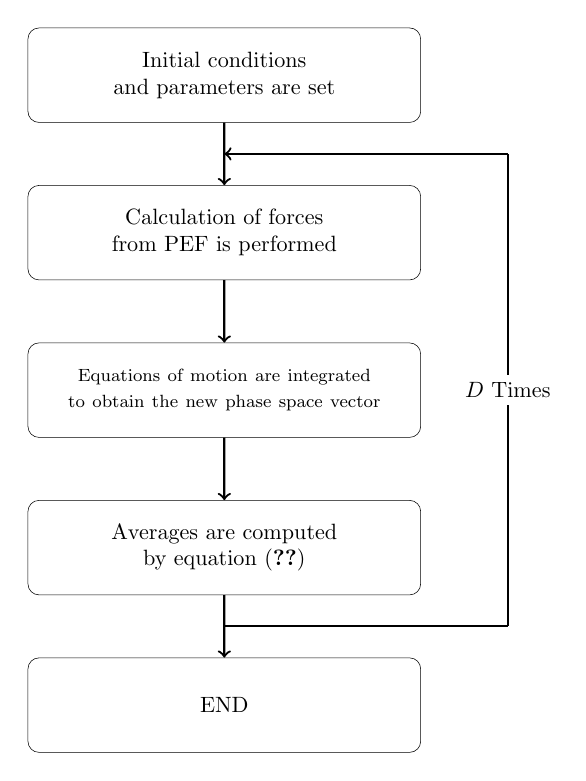
\begin{tikzpicture}[scale=0.8, transform shape]
	\node[rectangle,draw,rounded corners,very thin,minimum width=6cm,minimum height=1.5cm,text width=6cm,align=center] (A) at (0,10) {Initial conditions \\ and parameters are set};
	\node[rectangle,draw,rounded corners,very thin,minimum width=6cm,minimum height=1.5cm,text width=6cm,align=center] (B)  at (0,7.5) {Calculation of forces \\ from \ac{PEF} is performed};
	\node[rectangle,draw,rounded corners,very thin,minimum width=6cm,minimum height=1.5cm,text width=6cm,align=center] (C)  at (0,5) {\footnotesize Equations of motion are integrated to obtain the new phase space vector};
	\node[rectangle,draw,rounded corners,very thin,minimum width=6cm,minimum height=1.5cm,text width=6cm,align=center] (D)  at (0,2.5) {Averages are computed \\ by equation~(\ref{eq:MDTimeAve})};
	\node[rectangle,draw,rounded corners,very thin,minimum width=6cm,minimum height=1.5cm,text width=6cm,align=center] (E)  at (0,0) {END};
	\draw[thick,->] (A) -- (B);
	\draw[thick,->] (B) -- (C);
	\draw[thick,->] (C) -- (D);
	\draw[thick,->] (D) -- (E);
	\draw[thick,-] (0,1.25) -- (4.5,1.25);
	\draw[thick,-] (4.5,1.25) -- (4.5, 8.75) node[pos=0.5, fill=white] {$D$ Times};
	\draw[thick,->] (4.5, 8.75) -- (0, 8.75);
\end{tikzpicture}
\caption{Schematic representation of an MD simulation}
\label{fig:MDscheme}
\end{figure}

\subsection{Initial configuration}
Before a \ac{MD} simulation can be performed it is necessary to select an \textit{initial configuration}. The choice of it can be nontrivial and it depend on the complexity of the system, moreover, all the successive simulations depend on that initial configuration, so if that are wrong, maybe even the simulations produce wrong results. Then, carefully attention must be used to setting up the initial configuration.

Setting up an initial configuration mean to prepare a $N$--particle system and give all the particle's positions and velocities, i.e. give all the $6N$ coordinates of the initial phase space vector $\vec x_0$. The initial velocities can be extracted randomly from the Maxwell--Boltzmann distribution function at a specific system's temperature
\begin{equation*}
	f(v_i) = \sqrt{\frac{m_i}{2\pi k_B T}}e^{-\left ( \frac{m_iv_i^2}{2k_B T}\right )}
\end{equation*}
moreover the random assignment algorithm must rescale all the velocities such that the total system's momentum $\vec P = \sum_{k=1}^N m_k\vec v_k$ is zero, this is equivalent to a \ac{COM} motion removal. That is done because, in general, the total force acting on the system $\vec F = \sum_{k=1}^N F_i$ is zero, then the \ac{COM} motion is constant and to avoid a constant drift of the system in space this can be removed. Of course this is a constraint on the system and it must be take into account because it reduce the system's \ac{DOF} by $3$.

\subsection{Periodic boundary conditions}
In all experiment our systems is necessarily confined in to a box with some initial size. Even in a \ac{MD} simulation the sample system is inserted into a \textit{simulation box} whose shape can be differently chosen to better reproduce the symmetry of the simulated system. That box give us the trivial possibility to introduce a well defined reference system of coordinate in which respect the particles positions are assigned. Obviously we must not forget to correctly treat the \textit{boundary conditions}. In order to avoid the treatment of surface effect and for considering only a infinite bulk system, a \ac{PBC} are imposed to the simulation box. This, let us also the possibility to simulate the system's bulk proprieties without considering a large number of particles.
\begin{SCfigure}
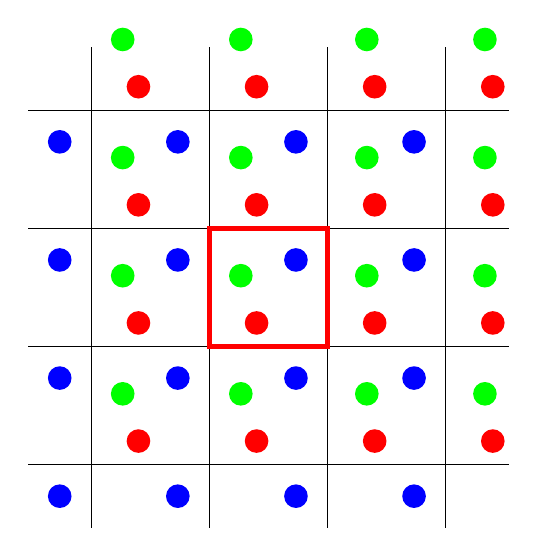
\begin{tikzpicture}
	\draw[step=1.5cm,thin] (-0.8,-0.8) grid (5.3,5.3);
	\draw[draw=red,ultra thick] (1.5,1.5) rectangle (3,3);
	\foreach \x in 	{0.6,2.1,3.6,5.1}
		\foreach \y in {0.3,1.8,3.3,4.8}
			\fill[fill=red] (\x,\y) circle (0.15);
	\foreach \x in 	{-0.4,1.1,2.6,4.1}
		\foreach \y in {-0.4,1.1,2.6,4.1}
			\fill[fill=blue] (\x,\y) circle (0.15);
	\foreach \x in 	{0.4,1.9,3.5,5}
		\foreach \y in {0.9,2.4,3.9,5.4}
			\fill[fill=green] (\x,\y) circle (0.15);
\end{tikzpicture}
\caption{Schematic view of a two--dimensional box with PBC imposed. The central, red contoured, box is the simulation box and it si replicated along each side.}
\label{fig:pbc}
\end{SCfigure}
To give a better idea, in figure~(\ref{fig:pbc}) is shown an example of a two--dimensional box with the \ac{PBC} imposed. The central, red contoured, box is the simulation box, the idea is to replicate that box in space along each sides so that there are no surface particles nor walls in the central box. When a particle moves in the central box, all its images virtually move the same way in the copies of the box so that if a particle leave the virtual boundary of the central box, then, its nearest image enters the box and the number density of particles in the simulation box is conserved. This virtual movement of image particles is achieved adjusting the positions of the simulation box particles which have left the main box. For example, is one use a cubic box and a particle crosses its boundary in one direction, say the $x$ direction, then its coordinate is corrected by subtracting (if leave the box in the positive direction) or adding the box side length parallel to $x$ direction. Even if the most used shape is the cubic one, not all the shapes are accessible to impose the \ac{PBC}, the most useful example is a spherical shape. When it is possible one have to use the most appropriate shape due to better describe the symmetry of the system, otherwise a closest approximation, compatible with \ac{PBC}, must be used.

Even if \ac{PBC} are used in a wide range of applications, it must be taken into account that imposing periodicity to a system may affect its properties. A clear limitation of the periodic cell is that it is not possible to achieve fluctuations that have a wavelength greater then the cells's length. This cause, obviously, the impossibility to sampling that vibrating modes. An other problem arises with the range of the inter--particles interactions: one have to choose carefully the size of the simulation box, or the number of particles if an $NPT$ ensemble is used, to ensure that the smallest simulation box length is greater then the interaction range. This can be made easily for example with the Van der Waals interaction. On the contrary is a difficult and time consuming task to do the same with the electrostatic interaction that are treated with more sophisticated methods (this will be better explained in the section~\ref{sec:longRangeInt}).

\subsection{Numerical integrators}
As we have seen above we need to solve numerically the equations of motion. Since the \ac{PEF} is a continuos function of the phase spaces vector at a time $t$, the simplest way is to use the so called \textit{finite difference} method. The basic idea is to expand the Newton's law in a Taylor series as follow
\begin{equation}
	\vec r_i(t + \delta t) = \vec r_i(t) + \vec v_i(t)\ \delta t + \frac{1}{2m_i}\vec f_i(t)\ (\delta t)^2\ +\ o((\delta t)^3)
	\label{eq:newtonTaylor}
\end{equation}
where we used the identities $\vec v_i(t) = \dot{\vec r}_i(t)$ and $m_i\ddot{\vec r}_i(t) = \vec f_i(t)$.

From this point, different algorithms have been developed. In the following we will describe in detail the most important, the \textit{Verlet algorithm}, and an its implementation the \textit{leap--frog algorithm}, which is the default used in our \ac{MD} tools for this thesis work.

\subsubsection{Verlet algorithm}
The Verlet algorithm required the positions and the forces at a time $t$ and the positions at a time $t-\delta t$ for calculate the  positions at a time $t+\delta t$. Starting from equation~\eqref{eq:newtonTaylor} we can write
\begin{align}
	\vec r_i(t+\delta t) &\simeq \vec r(t) + \vec v_i(t)\delta t + \frac{1}{2m_i}\vec f_i(t)\ (\delta t)^2
	\label{eq:verlet1} \\
	\vec r_i(t-\delta t) &\simeq \vec r(t) - \vec v_i(t)\delta t + \frac{1}{2m_i}\vec f_i(t)\ (\delta t)^2
	\label{eq:verlet2}
\end{align}
take its sum give us the new positions at a time $t+\delta t$
\begin{equation*}
	\vec r_i(t+\delta t) \simeq 2 \vec r_i(t) - \vec r_i (t - \delta t) + \frac{1}{2m_i}\vec f_i(t)\ (\delta t)^2
\end{equation*}
The velocities does not compare in the equation above and can be obtained taking the difference of equation~\eqref{eq:verlet1} and~\eqref{eq:verlet2}
\begin{equation*}
	\vec v_i(t) \simeq \frac{\vec r_i(t+\delta t) - \vec r_i(t-\delta t)}{2\delta t}
\end{equation*}
Since positions are computed as differences this is a fourth order algorithm and the precision is up to $(\delta t)^4$, but are also a sum of a small term (of the order $(\delta t)^2$) to the differences of two larger terms, this may cause a loss of precision.

The main disadvantage is that the velocities at a time $t$ are an output of the the calculation and not a part of the algorithm itself; moreover it is not self--starting because the algorithm required the positions at a time $t-\delta t$. At $t=0$ we need a trick for obtain the previous inexistent positions. The trick is to use the equation~\eqref{eq:verlet2} truncated at the first order: $\vec r_i(-\delta t) \simeq \vec r(0) - \vec v_i(0)\delta t$.

\subsubsection{Leap--Frog algorithm}
The leap--frog algorithm is a variant of the Verlet one and it is commonly implemented in many \ac{MD} tools, that is our case. It compute the positions at a time $t$ and the velocities at a time $t+\delta t/2$ from the forces at a time $t$ and the velocities at a time $t-\delta t$. The main advantage, respect to the Verlet algorithm, is that it is self--starting because not require the positions at a time $t-\delta t$.

First it calculate the velocities at a time $t+\delta t/2$ as follow
\begin{equation*}
	\vec v_i(t + \nicefrac{1}{2}\delta t) \simeq \vec v_i(t - \nicefrac{1}{2}\delta t) + \vec a_i(t)\delta t
\end{equation*}
then the positions at a time $t+\delta t$ are computed
\begin{equation*}
	\vec r_i(t + \delta t) \simeq \vec r_i(t) + \vec v_i(t + \nicefrac{1}{2}\delta t)\delta t
\end{equation*}
The velocities at a time $t$ can be calculated by
\begin{equation}
	\vec v_i(t) \simeq \frac{\vec v_i(t + \nicefrac{1}{2}\delta t) + \vec v_i(t - \nicefrac{1}{2}\delta t)}{2}
	\label{eq:lfVelocitiesSync}
\end{equation}

An other advantage is that the velocities are part of the algorithm itself and that it does not require the calculation of the difference between two large number, with an increasing of precision. The obviously disadvantage is that the positions and velocities are not synchronized and it require equation~\eqref{eq:lfVelocitiesSync} for calculating the velocities at a time $t$. The need to have velocities at the same time of positions, as for the Verlet algorithm, derived from the calculation of the kinetics energy contribution at the total energy: it must be computed with positions and velocities at the same time.
%Discorso energia cinetica nello stesso tempo delle posizioni

	\subsection{Neighbor list}
	\subsection{Thermostats algorithms} %Molecular Modelling, 382
			%Berendesen --> velocity rescale
	\subsection{Barostats algorithms} %Molecular Modelling, 382
		\subsubsection{Berendesen algorithm}

		\subsubsection{Parrinello--Rahman algorithm}

\section{Empirical Force--Field model}
As we have seen in the previous section \ac{MD} provides a variety of tools for solving the time evolution of a $N$--particle system to obtain its dynamics. Due to the possibility to capture different length and time scales \ac{MD} simulations can be used in a variety of systems, such a set of atoms, molecules or more complex system such as protein and macromolecules systems. In each of it systems, depending on the \textit{interaction model} and its \textit{parametrization}, we will be able to describe crucial molecular--level processes, such as hydrogen bond formation in organic molecules, which happen on the picoseconds time scale; or study slow processes such as the diffusion of massive colloidal particles, taking place on time scales of milliseconds if not seconds. When we study a soft or condensed matter system or, in general, a system composed by a large number of atoms (of the order of $N \gg 1000$), a crucial role play the \textit{Born--Oppenheimer approximation}. It says that we can separate the motion of the electrons by the motion of the atomic nuclei. That is done for integrating out the high frequency electrons' motions in order to remove some \ac{DOF}. Moreover the main interesting processes of soft and condensed matter, ranging from protein folding to glass transitions, from surface diffusion to ligand--receptor binding take place on longer time scales and involve larger number of atoms. Father if we want to know precisely the dynamics of the electrons in the system we have to introduce quantum mechanical methods that are, even for a small number of particles (of the order of $N\sim 100$), to much computationally time consuming, thus the Born--Oppenheimer approximation is indispensable. In the following, when we speak about atoms or chemical moieties we refer to it as for nuclei coordinates only without considering electrons at all.

Nevertheless atoms or molecules interactions, such as bond formation, is mediated by the electrons interactions. Thus, for describe the dynamics of such a system with a classical \ac{MD} tools and the Born--Oppenheimer approximation, it is necessary to develop an \textit{empirical model of the inter--atoms interactions} that mimic correctly the ``real'' interactions. Since forces are derived from the \ac{PEF} we need a model composed by the set of the simplest pairwise addictive potentials that mimic the inter--particles interactions. The model, the set of functional forms of the inter--particles interactions potential and its parametrization are collected in to the so called empirical \acf{FF}. The meaning of \textit{empirical} is that most of the functional forms of the inter--atoms interaction has no ``first principle'' justification and they are only an approximation to reality: there is not a correct way it are chosen as a compromise between accuracy and computational efficiency. Father it is necessary to stress out that a \ac{FF} is a well defined single entity containing the functional models of the interactions and also its parameterizations (and the way to obtain it). All the parameters of a \ac{FF} are in harmony to each other, change some parameters without retesting all the \ac{FF} is not allowed because, maybe, one can destroy the whole \ac{FF}.

For biomolecular applications exist two main classes of \acp{FF}: the \textit{atomistic} \acp{FF} which the basic particles are atoms, and the \textit{coarse--grained} \acp{FF} with the basic particles represent atom groups or a small chemical moieties. In this case, even the way to do the corse--graining of the atoms in the molecules, called \textit{mapping}, is part of the \ac{FF} itself. Different \ac{CG} \acp{FF} can use different mapping method even with the same functional forms.

In the latter we add some other informations about \acp{FF} and describe the principal functional forms for modeling the inter--particles interactions and how to treat it in a \ac{MD} simulation. For a more complete discussion about \acp{FF} the reader is addressed to the book by A. R. Leach \cite{Leach}. While in the next section we focus to the main \ac{CG} \ac{FF} used in this thesis work: the \textacr{MARTINI} \ac{CG} \ac{FF} developed by Marrink \etal\, [].

\paragraph{\textbf{\textacr{parameterization}}} In general the functional forms for potential interactions are common to all particles in the system, then the \ac{FF} is completed by a set of empirical parameters that characterize the interaction between different types of particles, whether they are atoms or whole chemical groups. Interaction parameters are empirical in the sense that it are assigned based on the reproduction of a small set of a target properties of a small group of systems. These target properties can be derived from experimental measurements or from finer--level calculations or simulations. Nowadays, atomistic and \ac{CG} biomolecular \acp{FF} come as ``packages'' of parameters and functional forms appropriate for the description of a large variety of chemical compounds in the liquid and solid phases.

\paragraph{\textbf{\textacr{transferability}}} As described above the parameterization of a \ac{FF} involves a small set of test systems for which some set of target proprieties are reproduced. The main characteristic of a \ac{FF} is the \textit{transferability} that means the ability of the model to describe more different situations that differ from those used at the parameterization stage. Of course one would expect to be able to make some predictions for a bigger variety of systems and for other proprieties not used in the parametrization stage. Common faults of organic \acp{FF} concern, for example, phase transitions of organic compounds and phase transitions temperatures.

\subsection{Inter--particles interactions}
For biomolecular applications the inter--particles interactions potential are divided in to two main classes: the \textit{bonded interactions} involving particles within the same molecules and the \textit{non--bonded interactions} engaging all particles in the system and commonly are only the Van der Waals and the electrostatic interactions. The most  common and general functional form for the \ac{PEF} is the following one
\begin{equation}
	\begin{aligned}
		U(\vec r_1, \cdots \vec r_N) = &\quad \frac{1}{2}\sum_{\text{bonds}} \frac{1}{2}k_i^b(l_i - l_{i0})^2\ + \frac{1}{2}\sum_{\text{angles}} k_i^a (\theta_i - \theta_{i0})^2\ +\\
		&+ \frac{1}{2}\sum_{\text{torsions}} V_n(1+\cos (n\omega - \gamma))\ + \\
		&+ \sum_{i=1}^N \sum_{j>i} \left ( {4\epsilon_{ij} \left ( \left ( \frac{\sigma_{ij}}{r_{ij}} \right )^{12} - \left ( \frac{\sigma_{ij}}{r_{ij}} \right )^6 \right )  + \frac{q_iq_j}{4\pi\varepsilon_0 r_{ij}}} \right )
	\end{aligned}
	\label{eq:FFPEF}
\end{equation}
The first two terms in equation~\eqref{eq:FFPEF} are harmonic potentials which model respectively the energy contribution due to deviation from reference bond length $l_{i0}$ and bond angle $\theta_{i0}$. Together with the bond and angle elastic constants, $k_{bi}$ and $k_{ia}$ respectively, they constitutes the set of parameters for bond and angle contributions. The angle contribution involve a set of three particles in the same molecule.  The middle line of equation~\eqref{eq:FFPEF} concern the energy contribution due to the bond's torsional change where $\omega$ is the
torsional angle. It involve four particles in the same molecule and mimic the energy barrier needed to rotate the bond angle along the bond axis. $\gamma$ is a phase factor, $V_n$ qualitatively describe the energy barrier for each $n$--th components and $n$ is defined as the number of minima for each components. The last line in equation~\eqref{eq:FFPEF} contains the energy contribution due to the non--bonded interactions: the Van der Waals modeled by a Lennard--Jones $12-6$ potential, fully characterized by the constants $\sigma_{ij}$ and $\epsilon_{ij}$ proper for each particles' pair; and the electrostatic potential described by the particles' charge $q$. The non--bonded interactions involve obviously all particles in the system, but for particles belonging to same molecule they are computed only if they  are separated by at least three bonds, i.e. if their interactions are not described by bonded terms. The various contributions described above are schematically represented in the figure~(\ref{fig:FFInteraction}).

\begin{figure}[!ht]
	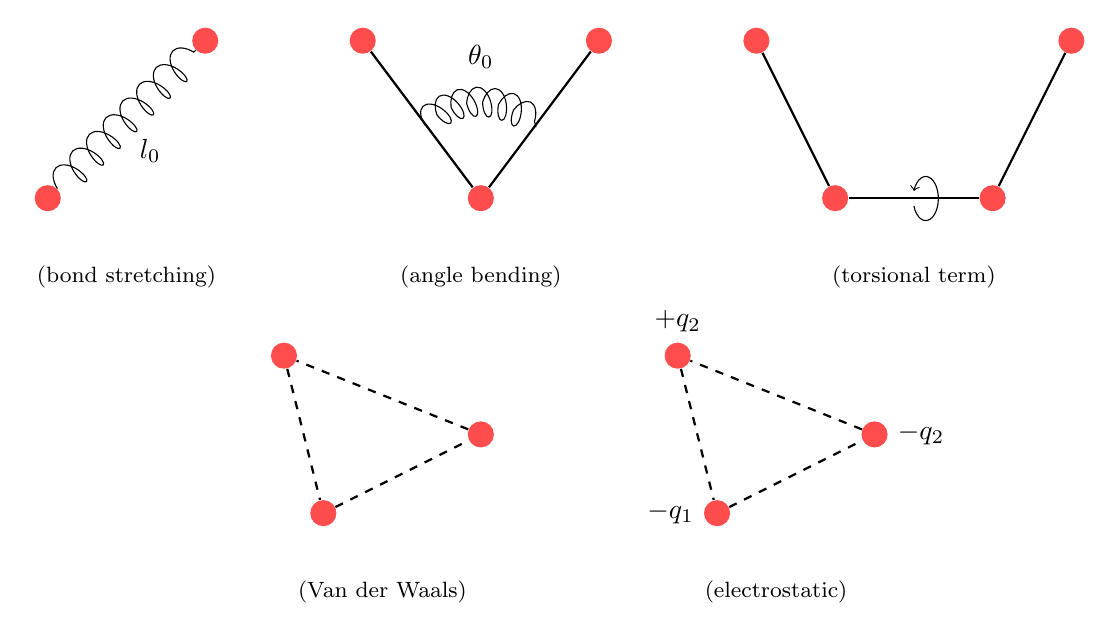
\begin{tikzpicture}
		%\draw[thin, gray!25] (0,0) grid (15,8);
		\node[fill=red!70, circle, radius=0.15] (1) at (0,6) {};
		\node[fill=red!70, circle, radius=0.15] (2) at (2,8) {};
		\draw[decorate, decoration={coil,segment length=3mm,amplitude=2mm}] (1) -- (2);
		\node[] at (1.3,6.6) {$l_0$};
		\node[] at (1,5) {\footnotesize(bond stretching)};
		\node[fill=red!70, circle, radius=0.15] (3) at (4,8) {};
		\node[fill=red!70, circle, radius=0.15] (4) at (5.5,6) {};
		\node[fill=red!70, circle, radius=0.15] (5) at (7,8) {};
		\draw[thick,-] (3) -- (4) node[midway] (mid1) {};
		\draw[thick,-] (4) -- (5) node[midway] (mid2) {};
		\draw[-,decorate, decoration={coil,segment length=2mm,amplitude=2mm}] (4.8,6.91924) to[out=45,in=135] (6.2,6.9);
		\node[] at (5.5,7.8) {$\theta_0$};
		\node[] at (5.5,5) {\footnotesize(angle bending)};
		\node[fill=red!70, circle, radius=0.15] (6) at (9, 8) {};
		\node[fill=red!70, circle, radius=0.15] (7) at (10, 6) {};
		\node[fill=red!70, circle, radius=0.15] (8) at (12, 6) {};
		\node[fill=red!70, circle, radius=0.15] (9) at (13, 8) {};
		\draw[thick,-] (6) -- (7);
		\draw[thick,-] (7) -- (8);
		\draw[thick,-] (8) -- (9);
		\draw[->] (11,5.9) arc [start angle=-160, end angle=160, x radius=0.16cm, y radius=0.28cm];
		\node[] at (11,5) {\footnotesize (torsional term)};
		\node[fill=red!70, circle, radius=0.15] (10) at (3,4) {};
		\node[fill=red!70, circle, radius=0.15] (11) at (3.5, 2) {};
		\node[fill=red!70, circle, radius=0.15] (12) at (5.5, 3) {};
		\draw[thick,dashed] (10) -- (11);
		\draw[thick,dashed] (11) -- (12);
		\draw[thick,dashed] (12) -- (10);
		\node[] at (4.25,1) {\footnotesize(Van der Waals)};
		\node[fill=red!70, circle, radius=0.15, label=above:$+q_2$] (13) at (8,4) {};
		\node[fill=red!70, circle, radius=0.15, label=left:$-q_1$] (14) at (8.5, 2) {};
		\node[fill=red!70, circle, radius=0.15, label=right:$-q_2$] (15) at (10.5, 3) {};
		\draw[thick,dashed] (13) -- (14);
		\draw[thick,dashed] (14) -- (15);
		\draw[thick,dashed] (15) -- (13);
		\node[] at (9.25,1) {\footnotesize(electrostatic)};
	\end{tikzpicture}
	\caption{Schematic representation of the common inter--atoms interactions for biomolecular applications: bond stretching, angle bending, torsional term, Van der Waals and electrostatic interactions.}
	\label{fig:FFInteraction}
\end{figure}

\subsection{Non--bonded interactions}
The bonded interactions, as we can see in equation~\eqref{eq:FFPEF}, are at \textit{fixed range}, meaning that it depended, for example, on equilibrium bond's length that is fixed. That is not for the non--bonded interactions because they depends on the inter--particles distance $r_{ij}$ and they decay to zero as a power of $r_{ij}^{-d}$. Depending on the power order $d$ compared to the system's size they are split into \textit{short range} and \textit{long range} interactions. Obviously the Lennard--Jones potential decay more rapidly then the electrostatic one; then, it is a short range interactions, while the electrostatic is a long range interactions.

\subsubsection{Cut--off and shift method}
Calculations of the non--bonded energy contributions is the most time consuming part of an \ac{MD} simulations. Moreover, they are pairwise interactions and scale as $N^2$. Especially for the short range interactions, various method are developed in order to speed--up the simulations. The \textit{cut--off} method is the most used to treat the short range interactions, but in same cases even the long range. Taking one particle, the general idea, is to evaluate the non--bonded interactions with all other particles that are closer to the first for a distance of $r_c$, called \textit{cut--off}, otherwise the interactions is set to $0$. That means that the new potential is of the form
\begin{equation*}
v^*(r) = \left \{
	\begin{aligned}
&v(r) & \quad & r \le r_c \\
&0    & \quad & r >   r_c
	\end{aligned} \right .
\end{equation*}

Doing that generate a discontinuity in potential itself and in the first derivative, i.e. in the forces; this is bad for energy conservation. A trick for solving the discontinuity of the potential and to improve the energy conservation is to apply even a \textit{shift} of the potential value at $r_c$, since it is a constant it not affect the forces. We have
\begin{equation*}
v^*(r) = \left \{
	\begin{aligned}
&v(r) - v(r_c) & \quad & r \le r_c \\
&0    & \quad  & r >   r_c
	\end{aligned} \right .
\end{equation*}
For solving even the discontinuity of the forces, that can cause some instability in a simulation, we need to consider a linear term proportional to the first derivative of the potential, such as
\begin{equation*}
v^*(r) = \left \{
	\begin{aligned}
&v(r) - v(r_c) - \left . \frac{dv(r)}{dr}\right |_{r_c}\ (r - r_c) & \quad & r \le r_c \\
&0    & \quad  & r >   r_c
	\end{aligned} \right .
\end{equation*}
Although, the shift methods make the potential quite different from the ``true'' and this make difficult to retrieve the correct thermodynamics proprieties. Thus, even it can solve some instability, it must be carefully used.

An other powerful method is the \textit{switch} method. The general idea is to consider two cut--off $r_{c1}$ and $r_{c2}$. If $r \le r_{c1}$ the ``true'' forms are used; while for $r > r_{c2}$ it is set to zero. For $r_{c1} < r \le r_{c2}$ a \textit{switching functions} is considered in order to \textit{smoothly} switch the potential to $0$.

\subsection{Van der Waals interactions}
The Van der Waals forces are a set of interactions that are divided in to two main contribution: an attracting interactions and a repulsive one. The main contribution to both is due to quantum dynamics effect of the electrons cloud interactions through the Pauli exclusion principle; and the instantaneous electrostatic interactions, even if both atoms are neutral, such as dipole--dipole, induced dipole--dipole and induced dipole--induced dipole interactions, in a more rigorous description even they should be treated quantum mechanically. To the attractive contribution there are also the London dispersion forces that involves polar and non--polar atoms and is due to the instantaneous multipoles interactions, and the hydrogen--bonding that is due to quantum effect, instantaneous electrostatic interactions and an entropic contribution.

The common model to treat the Van der Waals interactions is to use a Lennard--Jones potential, the $12-6$ is the most common but even the $9-6$ is used depending on the system. The general forms for a $12-6$ Lennard--Jones potential is the following
\begin{equation}
	v(r) = 4\epsilon\left ( \left ( \frac{\sigma}{r}\right )^{12}  - \left ( \frac{\sigma}{r} \right )^6 \right ) = \frac{C_{12}}{r^{12}} - \frac{C_{6}}{r^{6}}
	\label{eq:lj126}
\end{equation}
where $C_{12} = 4\epsilon\sigma^{12}$, $C_{6} = 4\epsilon\sigma^{6}$ and $r$ is the pairwise particles distance. $\epsilon$ is related to the absolute value of minimum while $\sigma$ is relented to distance at the minimum: $r_{\text{min}} = 2^{\nicefrac{1}{6}}\sigma$. That constant are proper for each particles pair type. The attractive contribution is due to the negative part proportional to $r^{-6}$; while the repulsive one is due to the positive part proportional to $r^{-12}$. In figure~(\ref{fig:LG12511}) there is a example plot of the function~()\eqref{eq:lj126} with $\epsilon = \sigma = 1$.
\begin{figure}[!ht]
\centering
	\begin{tikzpicture}
		\begin{axis}[samples=1000,domain=0:3,restrict y to domain =-2:2,axis x line=bottom,axis y line=center,xlabel={$r$},xmin=0,ymin=-1.5,ymax=1.5,xmax=3,ytick={-1.5,-1,...,1.5}]
			\addplot[very thick]plot (\x,{4/\x^(12)-4/\x^(6)});
			\addplot[dashed]plot (\x, {0});
		\end{axis}
		\node[] at (-1.4,3) {$v(r)$};
	\end{tikzpicture}
	\caption{Example plot of a Lennard--Jones function with $\epsilon = \sigma = 1$.}
	\label{fig:LG12511}
\end{figure}

The simplest and computational efficient way to treat a Lennard--Jones function, and in general all the short range interactions, is to use the cut--off method together with the shift or switch methods in order to obtain a continuous potentials and/or a continuous forces. As we can see from figure~(\ref{fig:LG12511}) the Lennard--Jones potential go to zero rapidly with distance: at $r \sim 2\sigma$ its value is less then $1\%$ of the value in $r \sim \sigma$. A good choose for the cut--off is then of the order of $r_c \sim 2\sigma \div 3\sigma$.

\subsection{Electrostatic interactions}
\label{sec:longRangeInt}
One of the most important long range interaction is the electrostatic forces. Despite the long range characteristic, for purely computational efficient reason, most of the \acp{FF} for biomolecular applications treat them in the same way as a short range interactions by a cut--off method\footnote{In general, for computational reason, it is a common choice to consider the some cut--off for Van der Waals and electrostatic interactions.}. Of course this is an approximations and can lead to a serious issue in that proprieties or systems that strongly depend on the electrostatic interactions. Most issue due to a non well treatment of the Coulomb interactions are related to, for example, develop of a good polar solvent model (a good treatment of the electrostatic proprieties of water is really important or biological application), consider the interactions of charged particle with polar solvent, transport processes of charged moieties, calculations of the electrostatic potential inside a macromolecules and so on. The loss of computational efficiency in the calculations of the electrostatic energy contribution is that it needs to take into account \textit{all particles} in a system, but we can not forget the \ac{PBC}: even all the infinity images of all particles need to be taken.

If we consider only the simulation box the energy contribution is
\begin{equation}
	U = \frac{1}{2}\sum_{i=1}^N\sum_{j\ne i}^N\frac{1}{4\pi\varepsilon_0}\frac{q_iq_j}{r_{ij}}
	\label{eq:electrostatic}
\end{equation}
where $q_i$ and $q_j$ are the charge, respectively, of particles $i$ and $j$ and $r_{ij}$ is the distance between $i$ and $j$. But we need also all image box. Supposing, for simplicity, that the box is a cubic shape of size $L$, then we can define a tern of integer numbers $(n_x,\ n_y,\ n_z)$, $n_i=0,1,2,\cdots$ so that the position of all other image box, respect to the central simulation box, is $\vec n = L (n_x,\ n_y,\ n_z)$. Then the energy contribution became
\begin{equation}
	U = \frac{1}{2}\ \sideset{}{'}\sum_{n_x,n_y,n_z}^{+\infty}\ \sum_{i=1}^N\sum_{j=1}^N\frac{1}{4\pi\varepsilon_0}\frac{q_iq_j}{\|\vec r_i - \vec r_j + \vec n \|}
	\label{eq:electrostaticImage}
\end{equation}
where the prime indicate that for $\vec n = 0$ i.e. the energy contribution of the simulation box, we need to exclude the self interaction term: so in third sum must be $j \ne i$.

As describe above, a cut--off method is a good easy way solution for solving equation~\eqref{eq:electrostatic} and some time it reproduce good results. However, the increasing of computers power can lead to develop more rigorous methods to solve equation~\eqref{eq:electrostaticImage}, even for very large system. The main problem is that the summation in equation~\eqref{eq:electrostaticImage} is \textit{conditionally convergent}\footnote{A conditionally convergent series contains both positive and negative terms such that the positive or negative term alone form both a divergent series. The sum of a conditionally convergent series depends on the order in which the positive and negative terms are considered.} and converges extremely slowly and need too terms that became too time consuming, especially for large system (of the order of $N \sim 3\cdot 10^4$). The most important methods developed for solving that problem are based on the \textit{Ewald Summation Method} (\acs{ESM}). We shall describe that used in this thesis work: the Ewald summations method itself and the \textit{Particle Mesh Ewald} (\acs{PME}) method. For a more complete discussion about the advanced methods developed to treat the electrostatic interactions for biological applications the reader is addressed to the Review by Cisneros \etal\, \cite{Cisneros} and for more technical detail to the book by D. Frenkel and B. Smit \cite{Frenkel}.
%Moreover for a more technical detail the reader is addressed to the work by Ewald \etal\, [] for what concern the \ac{ESM}, and to the work by Darden \etal\, [] for what concern the \ac{PME} method.

\subsubsection{Ewald summation method} %Molecular Modelling, 334
The \acf{ESM} is the first method, introduced by Ewald \etal
%L'articolo è in tedesco... Lo devo citare?
, for a correct treatment of the electrostatic energy contribution in an ionic crystal that ca be extended in the electrostatic interactions of a periodic charge density. The basic idea is to split the summation in equation~\eqref{eq:electrostaticImage} in two series both rapidly convergent. The method is based on the following identity
\begin{equation}
	\frac{1}{r} = \frac{f(r)}{r} + \frac{1 - f(r)}{r}
	\label{eq:ewaldTrick}
\end{equation}
the trick is to choose a function $f(r)$ that will deal the rapid variation of the $1/r$ term for small $r$ and the slow decay at long $r$; in that case the two series can rapidly converge.

\begin{figure}[!hb]
	\centering
	\subfloat[Real space]{%
		\begin{tikzpicture}[scale=0.8, transform shape]
			\begin{axis}[samples=1000,domain=-1:4,axis x line=center,axis y line=none,axis x line=none, xmin=-0.4,xmax=2.5,ymin=-2.5, ymax=2.5]
				\addplot[thick]plot (\x, {0});
				\addplot[]plot (\x, {exp(-9*\x*\x/0.1)});
				\addplot[]plot (\x, {exp(-9*(\x-2)^2/0.1)});
				\addplot[]plot (\x, {-exp(-9*(\x-1)^2/0.1)});
				\addplot[smooth] plot coordinates {(0,0) (0,-1.5)};
				\addplot[smooth] plot coordinates {(1,0) (1,1.5)};
				\addplot[smooth] plot coordinates {(2,0) (2,-1.5)};
			\end{axis}
		\end{tikzpicture}
	}%
	\qquad
	\subfloat[Reciprocal space]{%
		\begin{tikzpicture}[scale=0.8, transform shape]
			\begin{axis}[samples=1000,domain=-1:4,axis x line=center,axis y line=none,axis x line=none, xmin=-0.4,xmax=2.5,ymin=-2.5, ymax=2.5]
				\addplot[thick]plot (\x, {0});
				\addplot[]plot (\x, {-exp(-9*\x*\x/0.1)});
				\addplot[]plot (\x, {-exp(-9*(\x-2)^2/0.1)});
				\addplot[]plot (\x, {exp(-9*(\x-1)^2/0.1)});
			\end{axis}
		\end{tikzpicture}
	}%
	\caption{Schematic illustration of the \acl{ESM} charge distribution: in (a) point charges (represented by vertical lines) and the neutralizing Gaussian charge distribution; in (b) the counteracts Gaussian distribution.}
	\label{fig:ewald}
\end{figure}

The \ac{ESM} for electrostatic interactions is based, as illustrated in figure~(\ref{fig:ewald}), considering each point--like charges in the system surrounded by a neutralizing charge distribution of equal magnitude but opposite sign that decay rapidly to zero. Simplify the notation for a one dimensional system, the simplest functional form is a Gaussian distribution centered in the position $r_i$ of the point--like charge $q_i$, of the form
\begin{equation}
	\rho_i(r) = \frac{q_i\alpha^3}{\pi^{3/2}}e^{-\alpha^2 (r - r_i)^2}
\end{equation}
that obey the relation
\begin{equation*}
	\frac{q_i\alpha^3}{\pi^{3/2}}\int_{r_i-\epsilon}^{r_i+\epsilon}e^{-\alpha^2 (r - r_i)^2}\ dr \simeq q_i
\end{equation*}
where $(r_i-\epsilon; r_i+\epsilon)$ is a small interval around $r_i$. The energy contribution due to this set up, the point--like charge \textit{and} the gaussian charge distribution, is given by
\begin{equation}
	U_r = \frac{1}{2}\sum_{i=1}^N\sum_{j=1}^N\ \sideset{}{'}\sum_{n_x,n_y,n_z}\ \frac{q_iq_j}{4 \pi \varepsilon_0} \frac{\erfc{(\alpha \| \vec r_i - \vec r_j + \vec n \|)}}{\| \vec r_i - \vec r_j + \vec n \|}
	\label{eq:ewaldReal}
\end{equation}
where $\erfc{(x)} = 1-\erf{(x)}$ is the complementary error function and $\erf{(x)}$ is the error function given by
\begin{equation}
	\erfc{(x)} = \frac{2}{\sqrt{\pi}}\int_{x}^{+\infty} e^{-t^2}\ dt, \qquad \erf{(x)} = \frac{2}{\sqrt{\pi}}\int_{0}^{x} e^{-t^2}\ dt
	\label{eq:erf}
\end{equation}
The point is that the summation involving the complementary error function in equation~\eqref{eq:ewaldReal} is rapidly convergent and it need very few terms so that a cut--off method can be safety used. The rate of convergence depends on the $\alpha$ parameter, bigger is $\alpha$ more rapidly converge and shorter can be the cut--off.
Thus the \ac{ESM} use the $\erfc{r}$ as a $f(r)$ function in the equation~\eqref{eq:ewaldTrick}. Of course since we have add a non physical neutralizing charge distribution in the system we must consider an other distribution of equal magnitude but opposite sign in order to restore the real charge distribution of the system. In view of the identity in the equation~\eqref{eq:ewaldTrick} that is done considering a distribution of the form $(1-f(r))/r$ so, using equation~\eqref{eq:erf}, it is of the form $\erf{(r)}/r$. While the former it is compute in the \textit{real space}, an other trick, is to consider the latter energy contribution due the counteracts charge distribution of the neutralizing charge, in the \textit{reciprocal space}, thus considering its Fourier transform. That energy contribution is given by
\begin{equation}
	U_f = \frac{1}{2}\sum_{i=1}^N\sum_{j=1}^N\ \sum_{k_x,k_y,k_z}\ \frac{1}{4\pi\varepsilon_0}\frac{4\pi}{L^3k^2}e^{-k^2/(4\alpha^2)}e^{\mathsf{i}{\vec k \cdot (\vec r_i - \vec r_j)}}
	\label{eq:ewaldReciprocal}
\end{equation}
where $\vec k = 2\pi\vec n/L$ are the reciprocal vectors. Even this reciprocal sum converge rapidly as the summation in equation~\eqref{eq:ewaldReal}; then a cut--off method can be safety used. Nevertheless, as opposite to the former, smaller is the $\alpha$ shorter can be the cut--off. Clearly it need a proper \textit{balance} between the real and reciprocal space summation.

Since in equation~\eqref{eq:ewaldReal} even the self interaction with each Gaussian is included we need to add another item for cancel out it; that is done by the self--term
\begin{equation}
	U_{self} = -\frac{\alpha}{\sqrt{\pi}}\sum_{i=1}^N\frac{q_i}{4\pi\varepsilon_0}
	\label{eq:EwaldselfTerm}
\end{equation}

Summarizing, the energy contribution of the electrostatic interactions by the \ac{ESM}, is computed summing the equations~\eqref{eq:ewaldReal},\eqref{eq:ewaldReciprocal} and~\eqref{eq:EwaldselfTerm} to obtain
\begin{equation}
	\begin{aligned}
		U =&\quad\frac{1}{2}\sum_{i=1}^N\sum_{j=1}^N\ \sideset{}{'}\sum_{n_x,n_y,n_z}\ \frac{q_iq_j}{4 \pi \varepsilon_0} \frac{\erfc{(\alpha \| \vec r_i - \vec r_j + \vec n \|)}}{\| \vec r_i - \vec r_j + \vec n \|}\ + \\
		 &+ \frac{1}{2}\sum_{i=1}^N\sum_{j=1}^N\ \sum_{k_x,k_y,k_z}\  \frac{1}{4\pi\varepsilon_0}\frac{4\pi}{L^3k^2}e^{-k^2/(4\alpha^2)}e^{\mathsf{i}{\vec k \cdot (\vec r_i - \vec r_j)}}\ + \\
		 &- \frac{\alpha}{\sqrt{\pi}}\sum_{i=1}^N\frac{q_i}{4\pi\varepsilon_0}
	\end{aligned}
	\label{eq:EwaldEnergy}
\end{equation}
The first line is the real space contribution while the second is the Fourier energy contribution. Since the last self--interaction term is constant it does not affect forces computations. The \ac{ESM} offer a well defined method to properly treat the electrostatic interactions, nevertheless it is a quite expensive in term of computational resources. If $\alpha$ and the cut--off are constant, then the computation scales as $\sim N^2$; while if $\alpha$ and the cut--off are dynamically updated then it scales as $\sim N^{\nicefrac{3}{2}}$ but this can lead to an incompatibility between the Van der Waals interactions cut--off and the electrostatic one compromising the efficiency gain. Despite we have described that method applied to the electrostatic interactions, it can be used, with some changes, to all long--range interactions and in general to all energy contributions that decay as $r^{-d}$, for example, even with the Van der Waals energy contributions.

For biomolecular applications most \ac{MD} tools set an equal cut-off radius for both Van der Waals interaction the the real part of the Ewald summation~\eqref{eq:EwaldEnergy} in order to achieve for both a scaling of the order $\sim N$. However in this way the computation of the reciprocal part in the Ewald summation~\eqref{eq:EwaldEnergy} will be very inefficient and scales as $\sim N^2$. In order to increase the efficiency on the calculation of the Fourier transform a various of advanced methods can be used. It are all based on the use of the \ac{FFT} methods. In this way the reciprocal part can scales as $\sim N\ln N$. Since \ac{FFT} require discretize quantity, the idea of such method, called \textit{Particle Mesh} is to consider the charge density spread on a mesh grid and then evaluate the electrostatic potential via solving the Poisson's equation using fast Poisson solver together with \ac{FFT} method; that can be done, for example, exploiting the \ac{PBC} in order to discretize and make periodic the Poisson's equation.
Such algorithm include the \textit{particle--particle particle--mesh} method, \textit{Particle mesh Ewald} method, \textit{Fast--Fourier Poisson} method and a recent methodology based on multi--scale mesh grid; the efficiency and accuracy of such mesh--based algorithms depend strongly on the way in which the charges are attributed to mesh points, different for each methods. In the latter we describe the one used in this thesis work, the \acf{PME} method.

\subsubsection{Particle mesh Ewald method}
The \acf{PME} method developed by Darden \etal\, \cite{DardenPME} are based on the \ac{ESM} so the starting point is the equation~\eqref{eq:EwaldEnergy}. In which, as described above, the first part of the Ewals summation are computed in the real space together with the Van der Waals contributions using the same cut--off radius. While the reciprocal part are computed using \ac{FFT} methods, in order to have a gain of performance. For doing this, first, we need to consider a grid mesh in which the Gaussian counteracts charge density are spread into. The basic idea, then, is to achieve the electrostatic energy solving the Poisson's equation through \ac{FFT} methods. The efficiency and the accuracy depends on the way the charges are distributed into the grid. For doing this a \textit{charge assignment function}, $W(r)$ is introduced such that, considering for simplicity a one dimensional system, the fraction of a charge at position $r$ assigned to a grid point at position $r_p$ is given by $W(r_p - r)$. Hence, if we have a charge density $\rho(r)$ then the charges at the grid point $r_p$ are given by
\begin{equation}
	q_M(r_p) = \int_0^L\ W(r_p - r) \rho (r)\ dr
	\label{eq:meshAssign}
\end{equation}
where $L$ is the box length and, if $h$ is the grid spacing, $M = L/h$ is the number of mesh point. In figure~(\ref{fig:gidAssign}) is schematically represented the charge assignment. The assignment function should have the following proprieties: should be an even function and should be normalized in such a way that the sum of the fractional charges equals the total charge of the system. Moreover the best accuracy is obtained with a dense grid in order to reduce as much possible the discretization of the charges density. However the computational cost increases as the number of grid points! So it clearly need a balance between efficiency and accuracy.
\begin{SCfigure}
	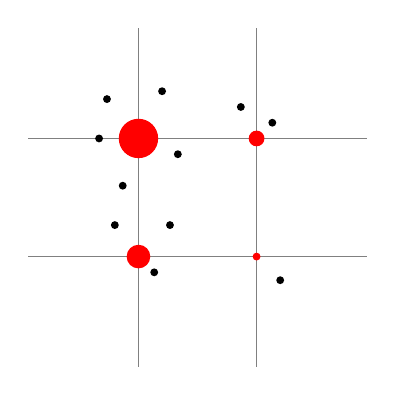
\begin{tikzpicture}
		\draw[gray,step=1.5] (0.1,0.1) grid (4.4,4.4);
		\fill[fill=red] (1.5,3) circle (0.25);
		\fill[fill=red] (3,1.5) circle (0.05);
		\fill[fill=red] (1.5,1.5) circle (0.15);
		\fill[fill=red] (3,3) circle (0.1);

		\fill[fill=black] (1, 3) circle (0.05);
		\fill[fill=black] (2, 2.8) circle (0.05);
		\fill[fill=black] (1.1, 3.5) circle (0.05);
		\fill[fill=black] (1.3, 2.4) circle (0.05);
		\fill[fill=black] (1.8, 3.6) circle (0.05);

		\fill[fill=black] (1.2, 1.9) circle (0.05);
		\fill[fill=black] (1.7, 1.3) circle (0.05);
		\fill[fill=black] (1.9, 1.9) circle (0.05);

		\fill[fill=black] (3.2,3.2) circle (0.05);
		\fill[fill=black] (2.8,3.4) circle (0.05);

		\fill[fill=black] (3.3,1.2) circle (0.05);
	\end{tikzpicture}
	\caption{A schematic representation of the charge assignment. The black filled circles are a unit particle charge, while the red one, are the charge assigned to grid points. Bigger is the circle, more is the charge.}
	\label{fig:gidAssign}
\end{SCfigure}

A nice way to solve the problem of charge assignment is to shift the problem in the discretization of the Fourier transform. It can be viewed as an interpolation problem. Consider the $e^{-\mathsf{i}\vec k\cdot \vec r_j}$ term in the Fourier transform of the equation~\eqref{eq:ewaldReciprocal}. In general $\vec r_j$ does not correspond to a mesh grid point, so that term is not part of a discrete Fourier transform. The idea, thus, is to interpolate it in terms of values of the complex exponential at the mesh points. Switching for simplicity to a one dimensional system, if the mesh grid has $M = L/h$ points, a particle coordinate $r_j$ is located between mesh points $[r_j/h]$ and $[r_j/h] + 1$ where $[]$ denote the integer part; thus a $p$--order interpolation of the exponential is of the form
\begin{equation*}
	e^{-\mathsf{i}kr_j} \simeq \sum_{i=1}^M W_{p}\left ( \frac{r_j}{h} - i \right ) e^{-\mathsf{i}khi}
\end{equation*}
where $W_{p}$ denote the interpolation coefficients. A $p$--order interpolation means that only the $p$ mesh points nearest the $r_j$ contributes to the sum. Assuming a point--like charge distribution the Fourier transform of the charge density is therefore
\begin{equation*}
	\rho_k \simeq \sum_{i}e^{-\mathsf{i}khi} \sum_j\ q_iW_{p} \left ( \frac{r_j}{h} - i \right )
\end{equation*}
we can interpret the above expression as the discrete Fourier transform of the charge density
\begin{equation*}
	\rho(i) = \sum_j\ q_iW_{p} \left ( \frac{r_j}{h} - i \right )
\end{equation*}
but using equation~\eqref{eq:meshAssign}, it is nothing that the point--like charge distribution assigned to the mesh point $i$ through the assignment function $W_{p}$.

We clearly see that the charge assignment problem is now shifted to the complex exponential interpolation. There are two main methods to make the interpolation: the \textit{Lagrange interpolation method} and the \textit{Euler SPLINE interpolation method}. The basic idea of the first is to use, as interpolating function, a polynomial function of degree $ \le (n-1)$ where $n$ is the number of points to interpolate, that passes through all the $n$ points, and it is constructed with a summation over the \textit{Lagrange basis polynomials} as follow
\begin{equation*}
	P(x) = \sum_{i=1}^n y_i \prod_{\substack{k=1\\k\ne j}}^n \frac{x-x_k}{x_j - x_k}
\end{equation*}
where $(x_i;y_i)$ are the set of points to interpolate. The main disadvantage of that method is that, even if $P(x)$ is continuous everywhere, its derivative is not, thus can lead to some instability in \ac{MD} simulations. The second method, that is the most used in \ac{MD} tools, is based on the concept of \textit{SPLINE interpolation}. Instead of using a unique interpolating function that passes to each points, the SPLINE method use a \textit{piecewise polynomial function}, called SPLINE, in which each pieces are smoothly connected and optimized to interpolate a subset of the points. The Euler SPLINE method use the \textit{exponential Euler SPLINE} that is constructed with the basis of the Euler $n$--degree polynomials $A_n(x;\lambda)$ generated by the following equation
\begin{equation*}
	\frac{\lambda - 1}{\lambda - e^z}e^{xz} = \sum_{n=0}^{+\infty} \frac{A_n(x;\lambda)}{n!}z^n
\end{equation*}
where $\lambda$ is a complex parameter and $z$ is a complex variable. The main properties of such SPLINE is that, it is $n-1$ times analytic continuously differentiable and then can solve the instability problem of the Lagrange interpolation method. In literature the former Euler SPLINE method is refers to \textit{smooth} \acl{PME} and the reader is addressed to the article by Essmann, Darder \etal\, \cite{EssmannSPME} for more technical detail about the interpolation procedure. 

Summarizing the \ac{PME} method is implemented following the latter procedure
\begin{itemize}
	\item By the interpolation of the complex exponential in the Fourier transform of the Ewald summation, the Gaussian counteracts charge distribution are spread into the mesh grid and a discretize Fourier transform are obtained;
	\item The Poisson's equations for the discretized charges are solved thought the \ac{FFT} methods;
	\item The reciprocal energy contribution are obtained considering the inverse Fourier transform; 
	\item Electrostatic forces are computed and assigned to the charged system's particles.
\end{itemize}
The main advantages of the \ac{PME} algorithm is that the potential energy and forces are smooth functions of the particles positions, offers a good energies conservations, offers a very well balance between accuracy and computational efficiency since it scales as $\sim N\ln N$ and it is easily generalizable to interaction potentials that decay as $r^{-d}$ such the Lennard--Jones potential. Nevertheless it not conserve very well the particles momentum due to \ac{RMS} errors in the forces calculations that have to be cancel out by removing the forces averages. 

\subsection{Charge representation}
Even if some methods are developed to speed up the electrostatic energy contribution such us the \ac{PME}, one of the main problem, related to the electrostatic interactions, of the \acp{FF} for biomolecular applications remains the \textit{charge representation}: the way that the charges of atoms or molecules are assigned to the system's particles. The problem arise from the representation of the negatively charged distribution due to the electrons cloud, that is, for instance a purely quantum effect, and the way that interactions of molecular electronic cloud can be achieved. Nevertheless that is crucial for a better description of the most electrostatic phenomena such us polarizability effect of molecules and polar solvent, solvation shell of charged ions, protein--ligands interaction, ion transport through polar and non--polar medium, self assembly processes and so on.

The mostly used solution is the \textit{atom--centered ``partial charge'' approximation} in which the full charge density of the molecule is replaced by a fractional point--like charges assigned to every atom. But now, one has to decide how much of the molecular charge density should be assigned to each atom. Traditionally most \acp{FF} assigned to each atom of a molecule a fixed partial--charge. The most used procedure for extracting the partial--charges from molecular wave functions are based on fitting that atomic charges with the molecular electrostatic potential, computed with \textit{ab initio} calculation such as \textit{density functional theory}. The fitting procedure consist of minimizing the deviation between the electrostatic potential produced by the charge assigned and the molecular electrostatic potential. Such representation are believed to be a an important source of error in the electrostatic treatment. Moreover with fixed charge assignment it is more challenging to take into account such phenomena that involve a transfer of charge inside the molecule, as polarization effect. The use of off--centered charges and/or higher order atomic multiples can significantly increase the treatment of electrostatic but of course it is necessary a good balance between accuracy and performance since the electrostatic problem can arise rapidly a loss of efficiency sometimes without a really gain in the accuracy.

\subsection{Polarization}
Polarization refers to the redistribution of the electron density of a molecule in the presences of an external electric field, generated, for example, by charged ions or an other molecule. The polarization effect generate non--addictive, attractive, inter-- or intra--molecular interactions that rapidly became a many--body interactions with even the induced polarization effect. It is recognized as an important physical effect and an increasing number of studies shows that the lack this effect can be a serious limitation, particularly, for ionic systems and chemical process that involve different environment such us water--protein or water--lipid membrane environment. In \ac{MD} simulations the polarization effect are included using either \textit{implicit} or \textit{explicit} method.

The implicit methods completely avoids the many--body calculation by including a mean polarization effect in the functional form of the interactions potential. The general idea is to surround all the simulation box by a transparent medium with a constant electrical permittivity $\varepsilon_r$. In this way the polarization effect is take into account considering a mean field theory and solving the Poisson's equation, for determine the electrostatic potential due to system's charges, by the substitution $\varepsilon_0\rightarrow\varepsilon_0\varepsilon_r$. If that method give an incomparable gain in performance, must be carefully used. The main disadvantage is that the mean polarization effect is add to all system's particles. That can be interesting, for example, when our system is composed principally by water; but if the simulation box is composed by a different chemical environments such as water and lipids or other organic matters, the electrical permittivity can not be the same, that can lead to a serious incorrect results of the proprieties of the organic matters and maybe of the simulation etall.

The way to correct the above behavior is to use an explicit methods. As the name suggest, the polarization effect is take into account for every molecules or solvent in the system by an its proper model included in the \ac{FF}. The general idea is to add to a molecule or atom some more internal \ac{DOF} for take into account the movement of charges and/or split the point--like charge assigned, for example, to a chemical group, to a partial charge assigned to each particles of the chemical group itself. That can be done for every molecules or atoms in the system and thus it is an optimum for better describe systems with different chemical environments.


\subsection{Atomistic model}
\subsection{Coarse--Grained model}

\section{MARTINI: a Coarse--Grained Force--Field}
	\subsection{Mapping}
	\subsection{Parametrization}
	\subsection{Bonded interaction}
	\subsection{Non--bonded interactions}
	\subsection{Simulation parameters}
	\subsection{Polarizable Water model}
	\subsection{Applications}

\section{Advanced sampling methods}
	\subsection{Metadynamics}

	\subsection{Umbrella sampling} %Molecular Modelling, 581
	
	
%Manuale GROMACS 3.17.5 PP/PME ranks
